\documentclass[a4paper,12pt]{article} 

%%% Работа с русским языком
\usepackage{cmap}                           % поиск в PDF
\usepackage{mathtext} 			 	       % русские буквы в формулах
\usepackage[T2A]{fontenc}               % кодировка
\usepackage[utf8]{inputenc}              % кодировка исходного текста
\usepackage{caption} %заголовки плавающих объектов
\captionsetup[table]{justification=centering} %установки для заголовков таблиц
\usepackage{tabularx}
\usepackage[english,russian]{babel}  % локализация и переносы
\usepackage[left=2cm,right=2cm,
    top=2cm,bottom=3cm,bindingoffset=0cm]{geometry}
\usepackage{wrapfig}
\usepackage{gensymb}
\usepackage{textcomp}
\usepackage{multirow}
\usepackage{pgfplots}
\usepackage{amsmath,amsfonts,amssymb,amsthm,mathtools} % AMS
\usepackage{euscript}	 % Шрифт Евклид
\usepackage{mathrsfs} % Красивый матшрифт
\usepackage{graphicx}%Вставка картинок правильная
\usepackage{float}%"Плавающие" картинки
\usepackage{wrapfig}%Обтекание фигур (таблиц, картинок и прочего)
\title{Лабораторная работа 4.3.2

Дифракция на ультразвуковых волнах}
\author{Кагарманов Радмир Б01-106}
\date{3 мая 2023 г.}

\begin{document}
\maketitle
\thispagestyle{empty}
\newpage
\setcounter{page}{1}

\paragraph{Цель работы:} изучение дифракции света на синусоидальной акустической решетке и
	наблюдение фазовой решетки методом темного поля.
	
	\paragraph{Оборудование:} оптическая скамья, осветитель, два длиннофокусных объектива, кювета с жидкостью, кварцевый излучатель с микрометрическим винтом, генератор звуковой частоты, линза, вертикальная нить на рейтере, микроскоп.
	
 \paragraph{Теоретическое введение\\}

	
	При прохождении ультразвуковой волны через жидкость в ней возникают периодические неоднородности коэффициента преломления, создается фазовая решетка, которую мы считаем неподвижной ввиду малости скорости звука относительно скорости света. Показатель
	преломления n изменяется по закону:
	
	\begin{equation}\label{}
	n = n_0 (1 + m \cos \Omega x)
	\end{equation}
	
	Здесь $ \Omega = 2 \pi / \Lambda $ --- волновое число для ультразвуковой волны, $ m $ --- глубина модуляции $ n $ $ (m \ll 1 $).
	
	Положим фазу $ \phi $ колебаний световой волны на передней стенке кюветы равной нулю, тогда на задней поверхности она равна:
	
	\begin{equation}\label{}
	\phi  = k n L = \phi_0 (1 + m \cos \Omega x)
	\end{equation}
	
	Здесь $ L $ --- толщина жидкости в кювете, $ k = 2 \pi / \lambda $ --- волновое число для света.
	
	После прохождения через кювету световое поле есть совокупность плоских волн, распространяющихся под углами $ \theta $, соответствующими максимумам в дифракции Фраунгофера:
	
\begin{equation}\label{}	
	\Lambda \sin \theta_m = m \lambda
\end{equation}

	Этот эффект проиллюстрирован на рисунке 1.
	\begin{figure}[h!]
		\centering	
		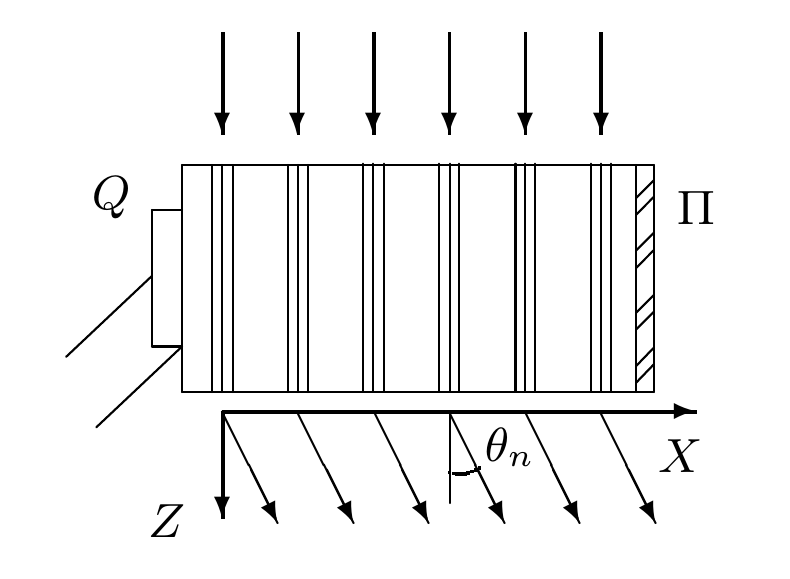
\includegraphics[width=0.3\textwidth]{difraction.png}
		\caption{Дифракция световых волн на акустической решетке}
		\label{diff}
	\end{figure}

	Зная положение дифракционных максимумов, по формуле (1) легко определить длину ультразвуковой волны, учитывая малость $ \theta $: $ \sin \theta \approx \theta \approx l_m /F  $, где $ l_m $ --- расстояние от нулевого до последнего видимого максимума, $ F $ --- фокусное расстояние линзы. Тогда получим:
	
	\begin{equation}\label{}
	 \Lambda = m \lambda F/ l_m 
	\end{equation}
	Скорость ультразвуковых волн в жидкости, где $ \nu $ --- частота колебаний излучателя:
	
\begin{equation}\label{}
	v = \Lambda \nu 
\end{equation}

Схема установки приведена на рисунке 2. Источник света Л через светофильтр Ф и конденсор К освещает вертикальную щель $ S $, находящуюся в фокусе объектива $ O_1 $. После объектива параллельный световой пучок проходит через кювету С перпендикулярно акустической решетке, и дифракционная картина собирается в фокальной плоскости объектива $ O_2 $ , наблюдается при помощи микроскопа М.

Предварительную настройку установки произведем в соответствии с инструкцией с зеленым фильтром, далее в работе используется красный.

	\begin{figure}[!h]
	\centering	
	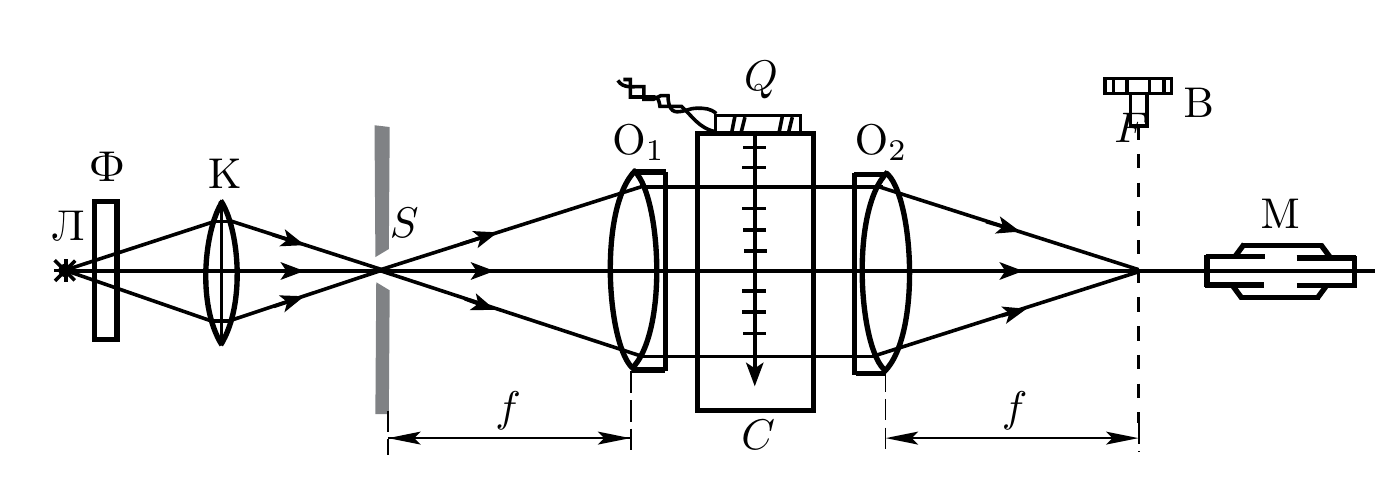
\includegraphics[width=0.7\textwidth]{shema1.png}
	\caption{Схема для наблюдения дифракции на акустической решетке}
	\label{shema1}
\end{figure}

\paragraph{Обработка результатов\\}
\subparagraph{1.} Параметры установки: фокусное расстояние объектива $  O_2  $ $ F = 30 $ см, одно деление винта микроскопа составляет 4 мкм.\par
Измерим положения $ x_m $ дифракционных максимумов с помощью микроскопического винта для четырех частот. Результаты измерений занесены в таблицы 1-4 ниже. На основе каждой таблицы построены графики зависимости $ x_m (m) $, они изображены на рисунках 3-6. С помощью формул (4) и (5) вычислим скорость ультразвука в воде.


\begin{table}[!h]
\begin{center}
\begin{tabular}{|c|c|c|c|c|c|c|c|}
\hline
     m & -3 & -2& -1 & 0 & 1 & 2 & 3 \\ \hline
     $x_m$, мкм & -97,5 & -59 & -29 & 0 & 31 & 69 & 104  \\ \hline
\end{tabular}
\end{center}
\caption{Измерение координаты $ m $-ого максимума $ x_m $ дифракционной картины при частоте генератора $ \nu = $ 1,048 МГц}
\end{table}
\begin{figure}[!h]
		\centering	
		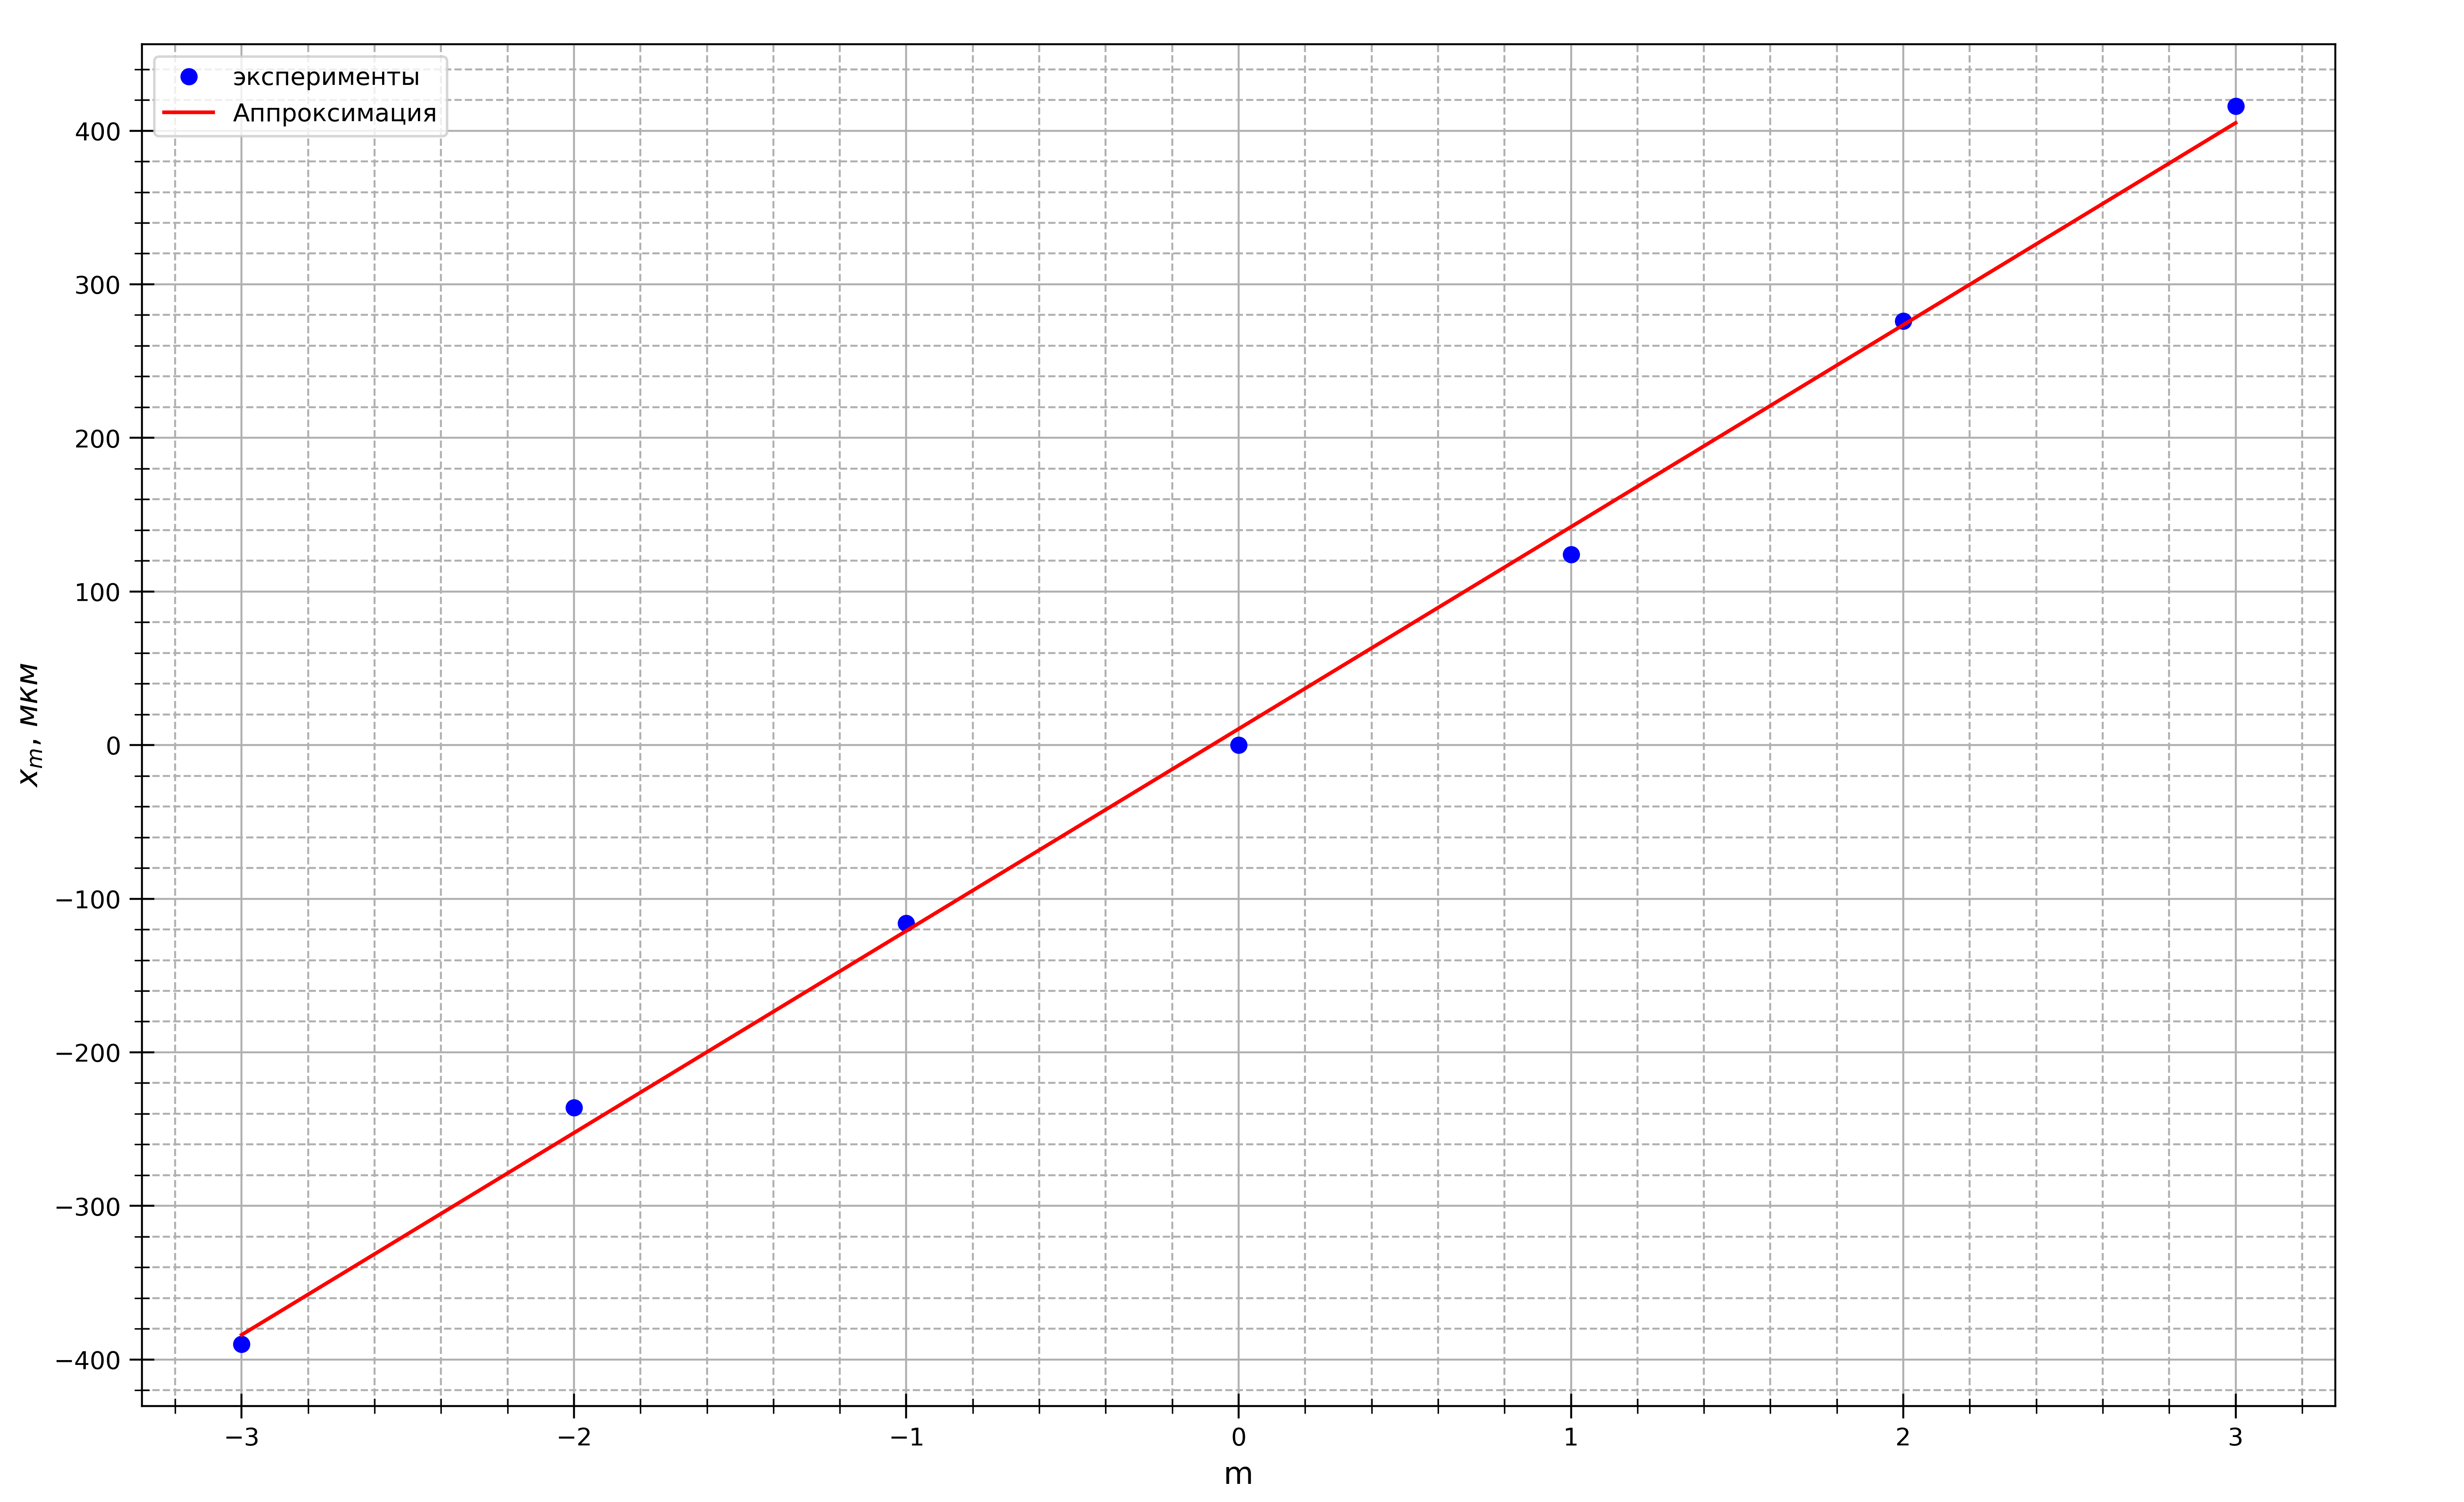
\includegraphics[width=0.7\textwidth]{graph1.png}
		\caption{Координаты $ m $-ого максимума $ x_m $ дифракционной картины при частоте генератора $ \nu = $ 1,048 МГц}
		\label{diff}
	\end{figure}
\begin{center}
    $v_1= 1530\pm 54$ м/c
\end{center} \newpage

\begin{table}[!h]
\begin{center}
\begin{tabular}{|c|c|c|c|c|c|c|c|}
\hline
     m & -3 & -2& -1 & 0 & 1 & 2 & 3 \\ \hline
     $x_m$, мкм & -108 & -68 & -37 & 0 & 30 & 61 & 98  \\ \hline
\end{tabular}
\end{center}
\caption{Измерение координаты $ m $-ого максимума $ x_m $ дифракционной картины при частоте генератора $ \nu = $ 1,179 МГц}
\end{table}
\begin{figure}[h!]
		\centering	
		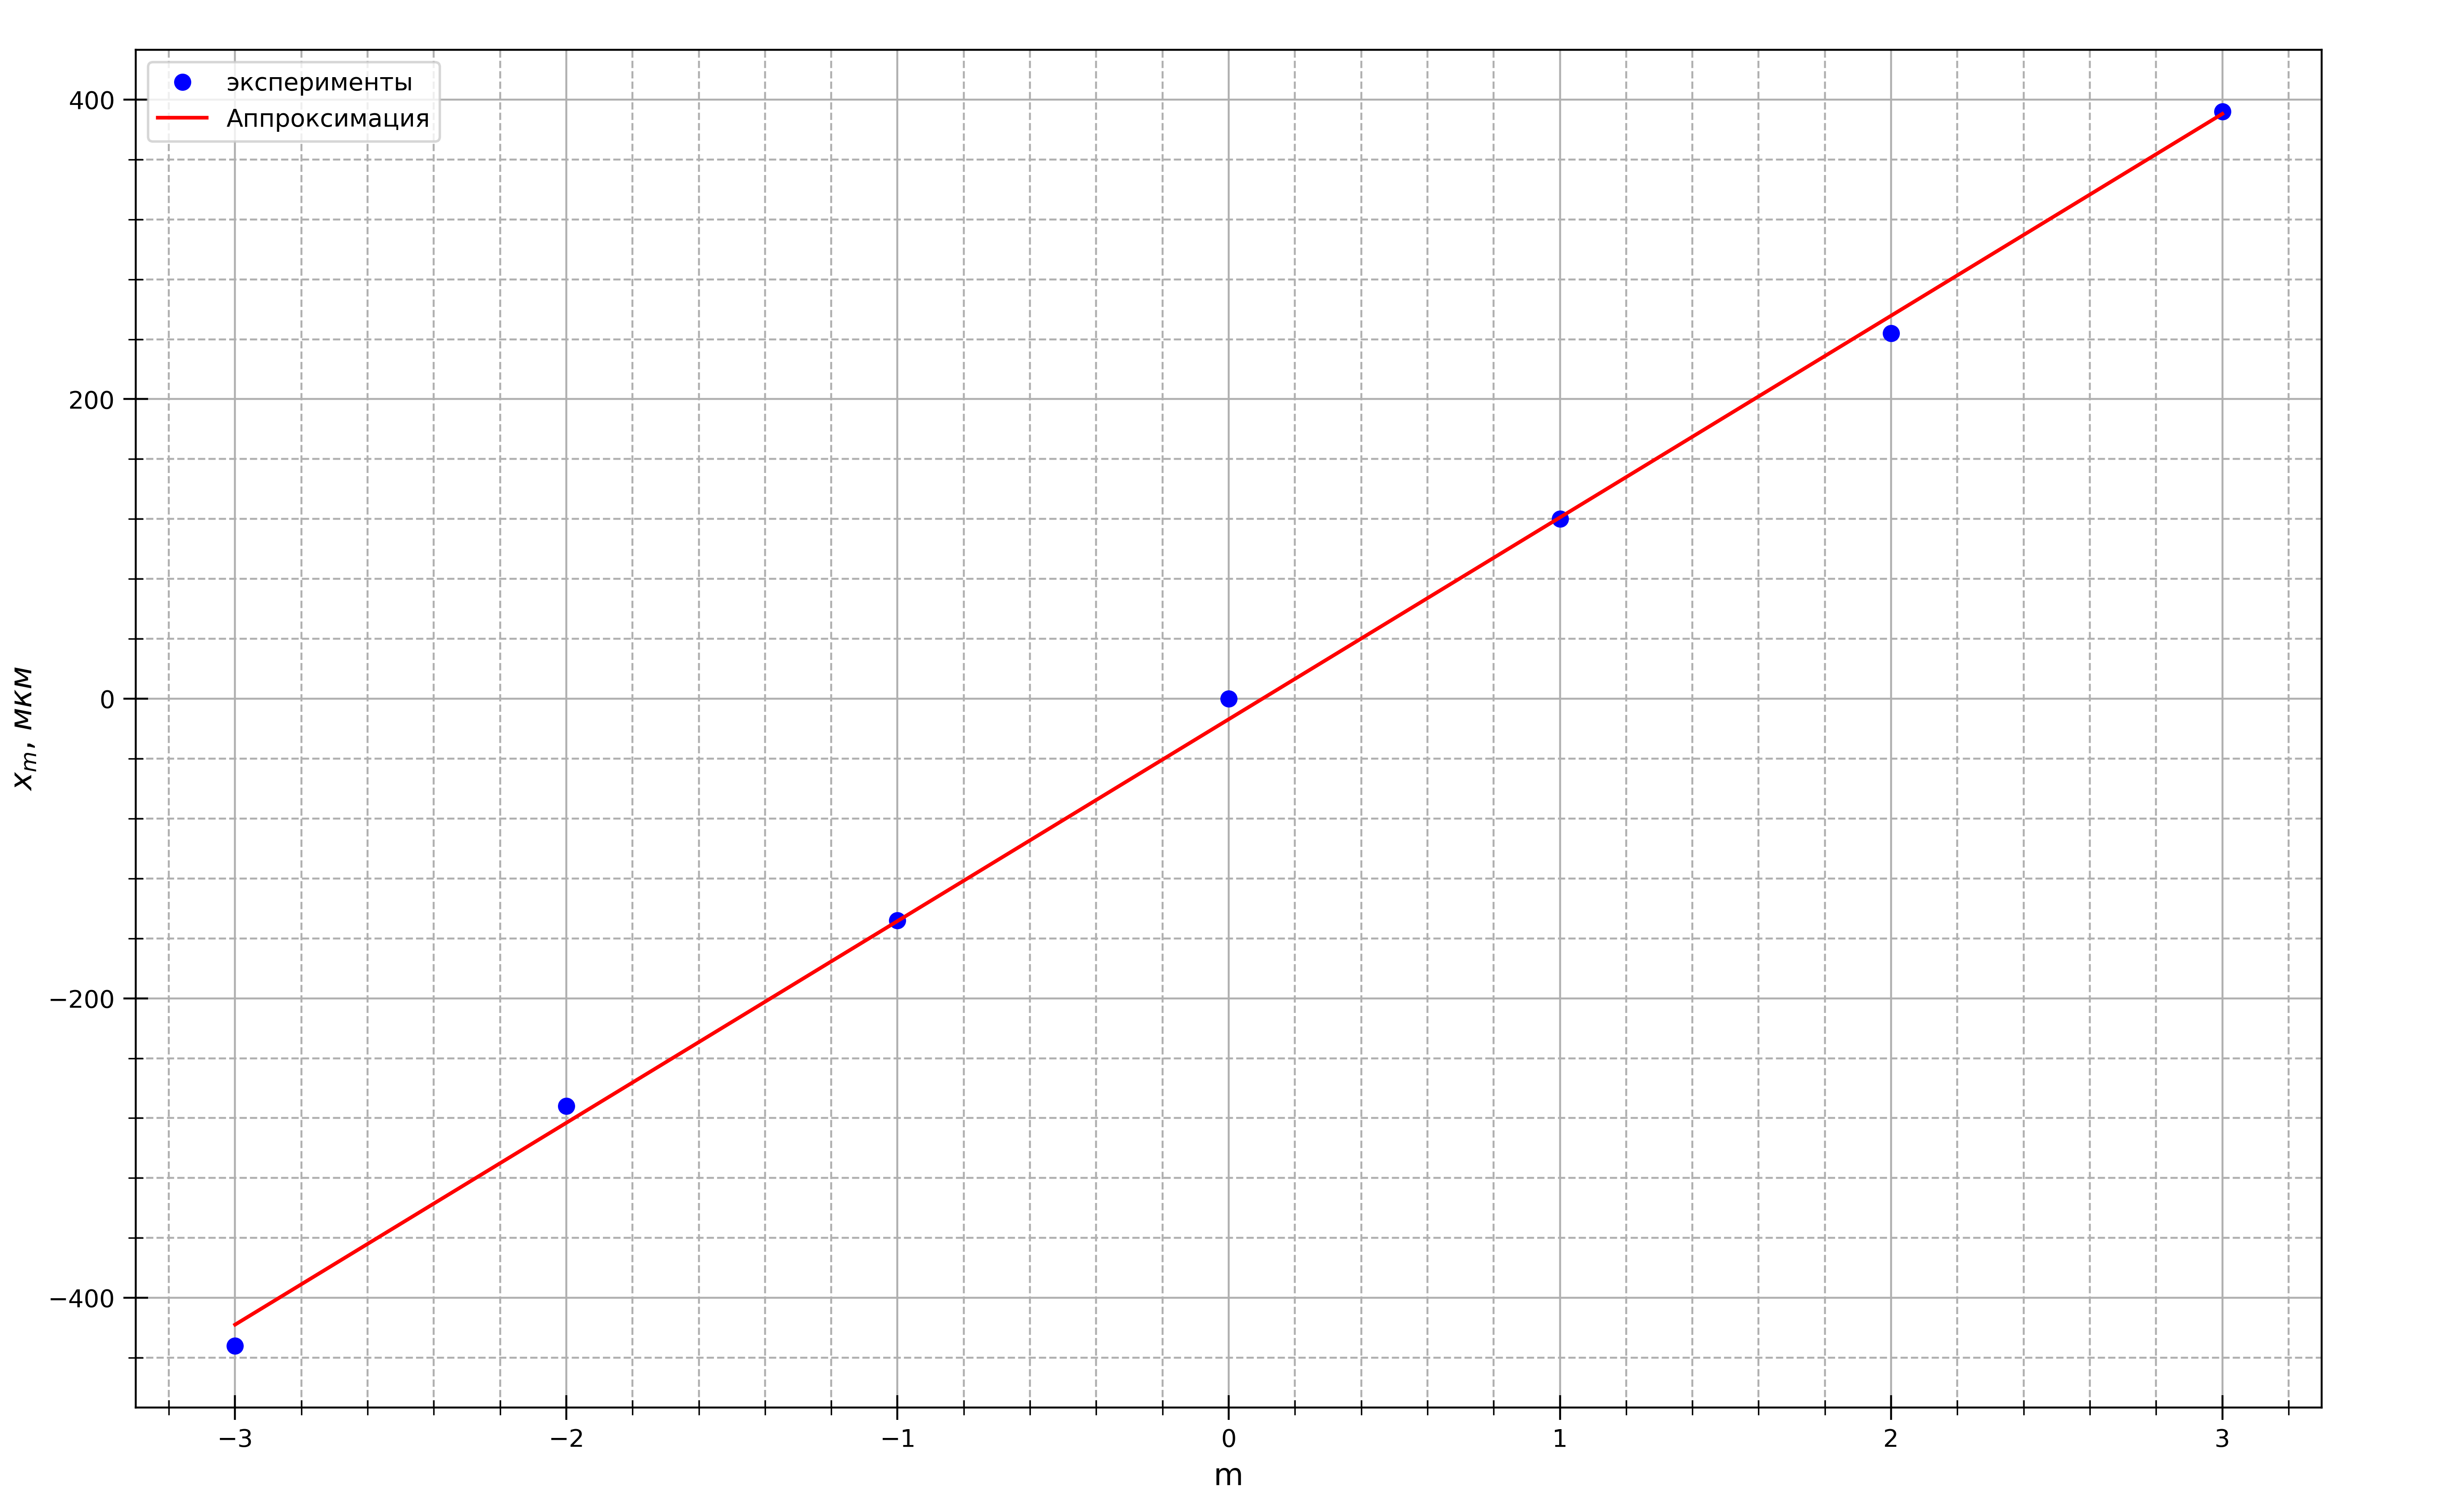
\includegraphics[width=0.7\textwidth]{graph2.png}
		\caption{Координаты $ m $-ого максимума $ x_m $ дифракционной картины при частоте генератора $ \nu = $ 1,179 МГц}
		\label{diff}
	\end{figure}
\begin{center}
    $v_2= 1680\pm 59$ м/c
\end{center}

\begin{table}[!h]
\begin{center}
\begin{tabular}{|c|c|c|c|c|c|c|c|}
\hline
     m & -3 & -2& -1 & 0 & 1 & 2 & 3 \\ \hline
     $x_m$, мкм & -274 & -178 & -90 & 0 & 79 & 161 & 261  \\ \hline
\end{tabular}
\end{center}
\caption{Измерение координаты $ m $-ого максимума $ x_m $ дифракционной картины при частоте генератора $ \nu = $ 2,883 МГц}
\end{table}
\begin{figure}[!h]
		\centering	
		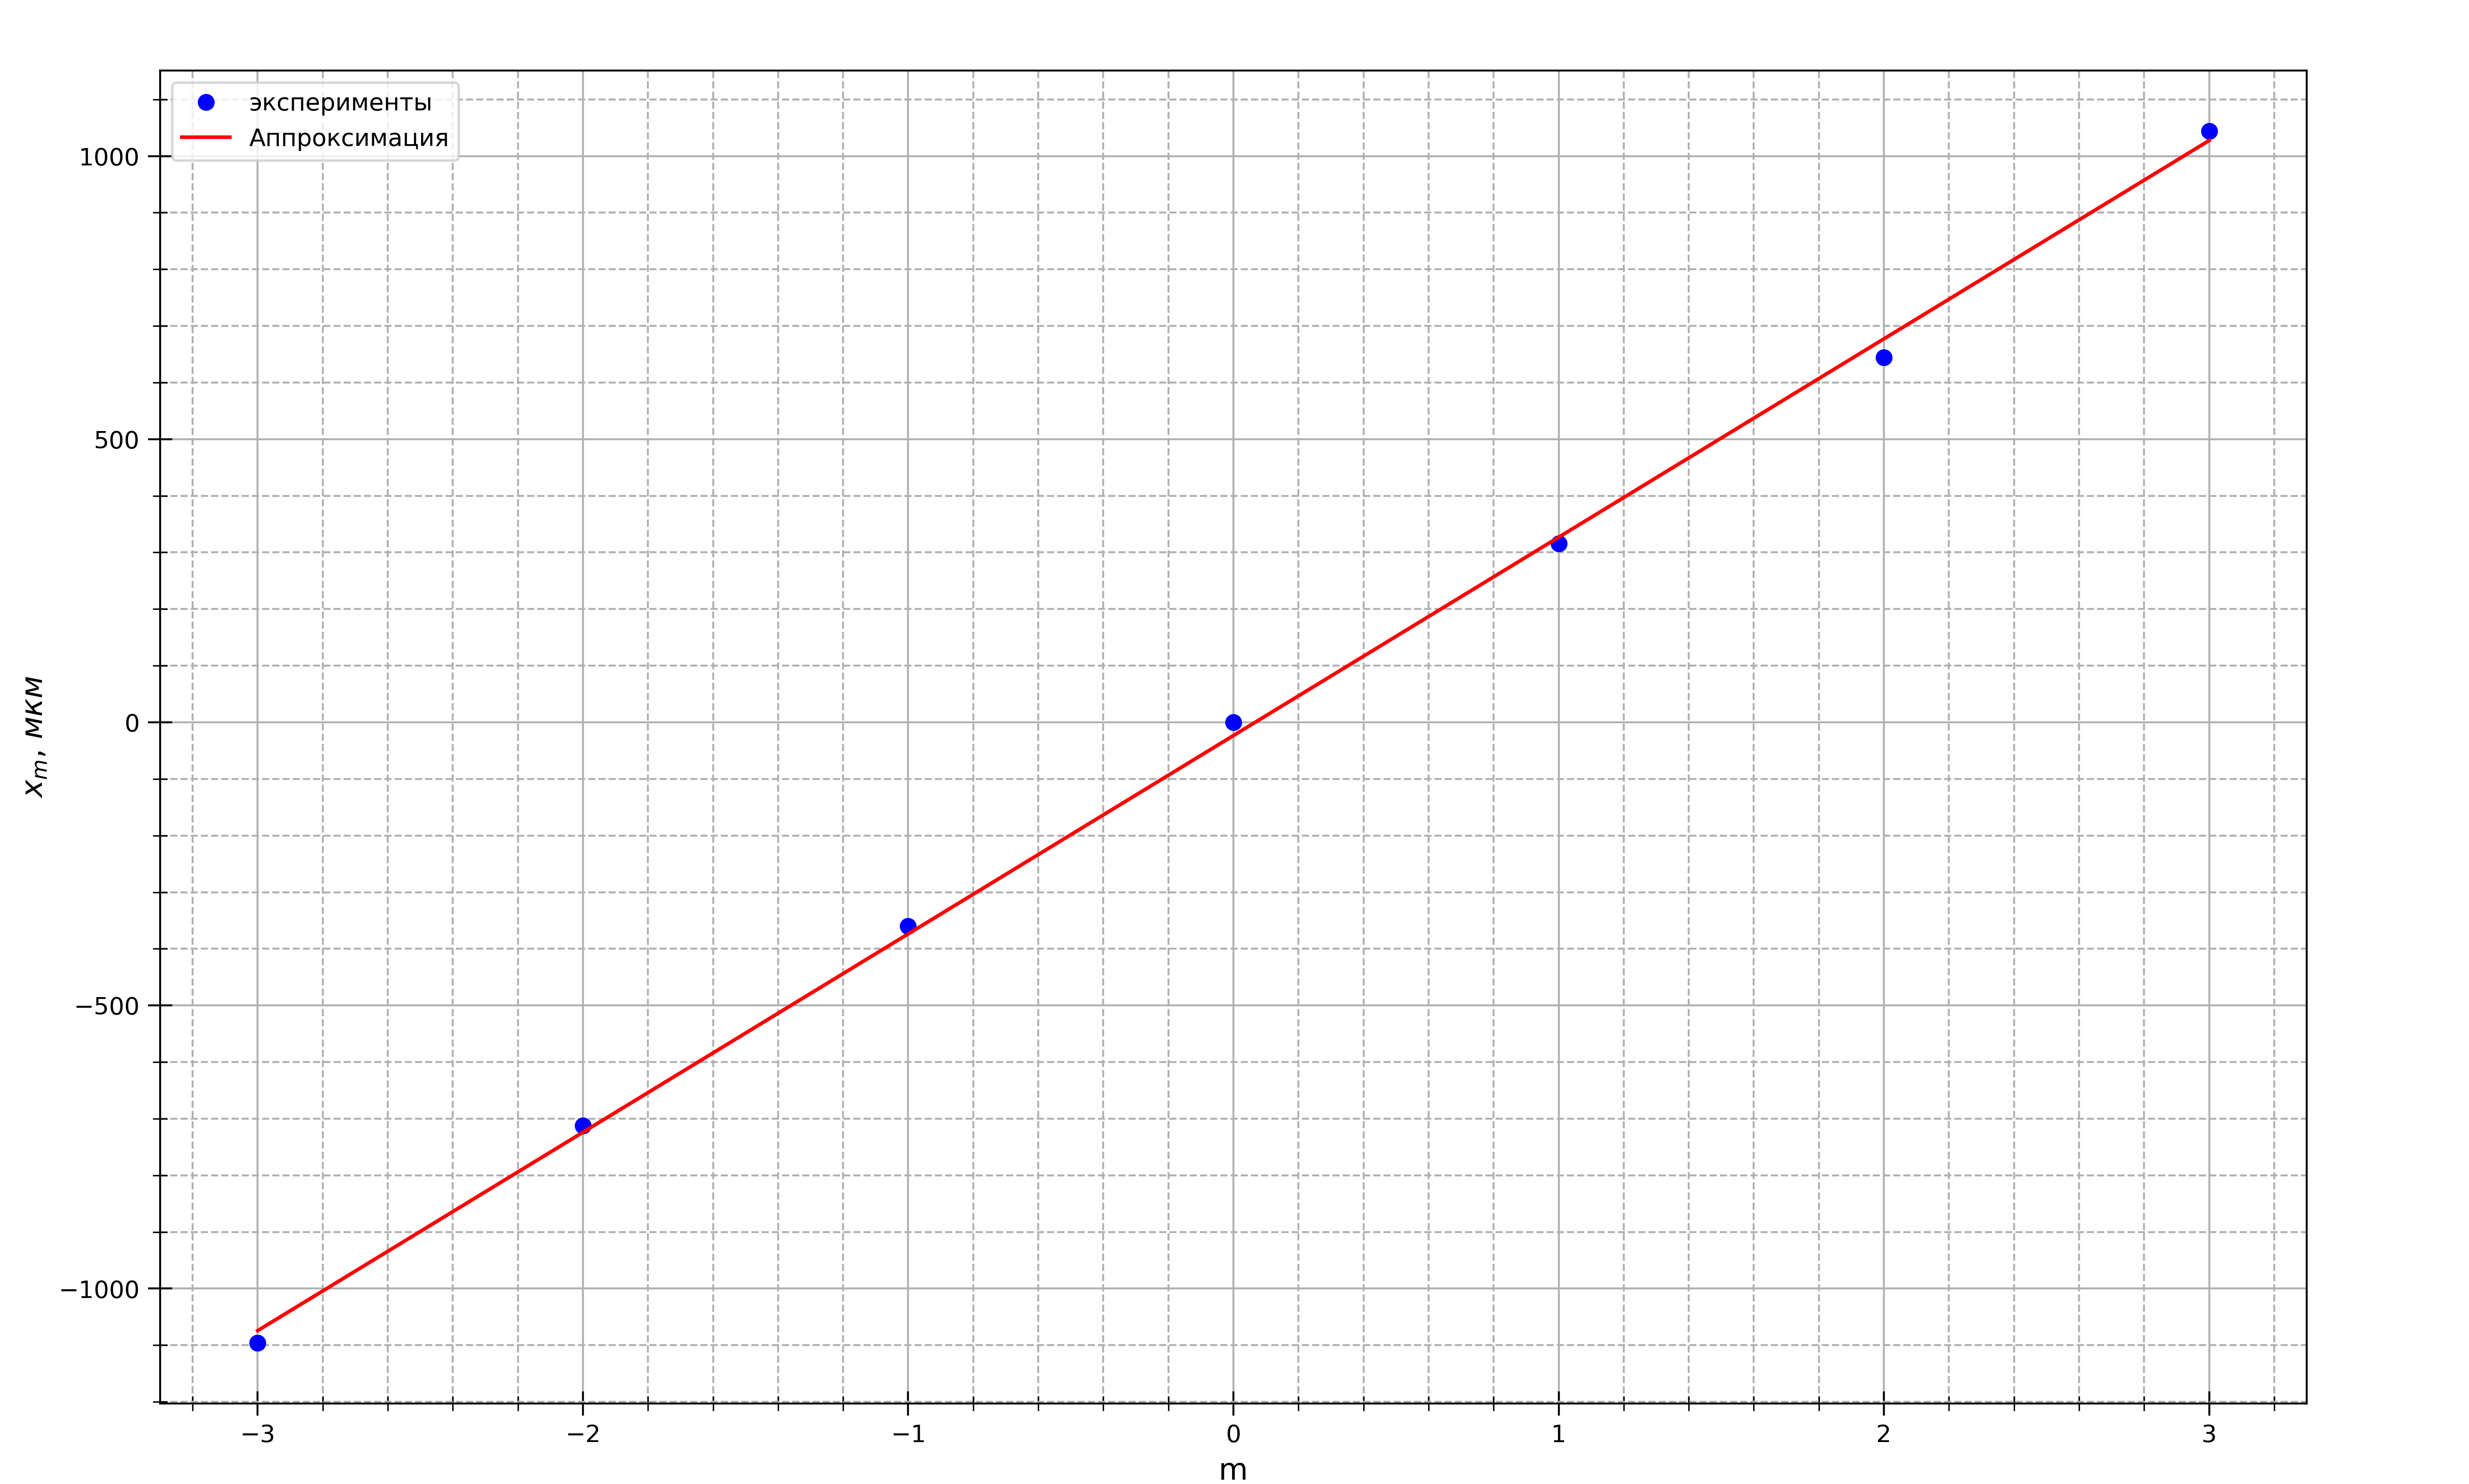
\includegraphics[width=0.7\textwidth]{graph3.png}
		\caption{Координаты $ m $-ого максимума $ x_m $ дифракционной картины при частоте генератора $ \nu = $ 2,883 МГц}
		\label{diff}
	\end{figure}
\begin{center}
    $v_3= 1582\pm 55$ м/c
\end{center}

\begin{table}[!h]
\begin{center}
\begin{tabular}{|c|c|c|c|}
\hline
     m & -1 & 0 & 1 \\ \hline
     $x_m$, мкм & -142 & 0 & 141  \\ \hline
\end{tabular}
\end{center}
\caption{Измерение координаты $ m $-ого максимума $ x_m $ дифракционной картины при частоте генератора $ \nu = $ 4,615 МГц}
\end{table}
\begin{figure}[!h]
		\centering	
		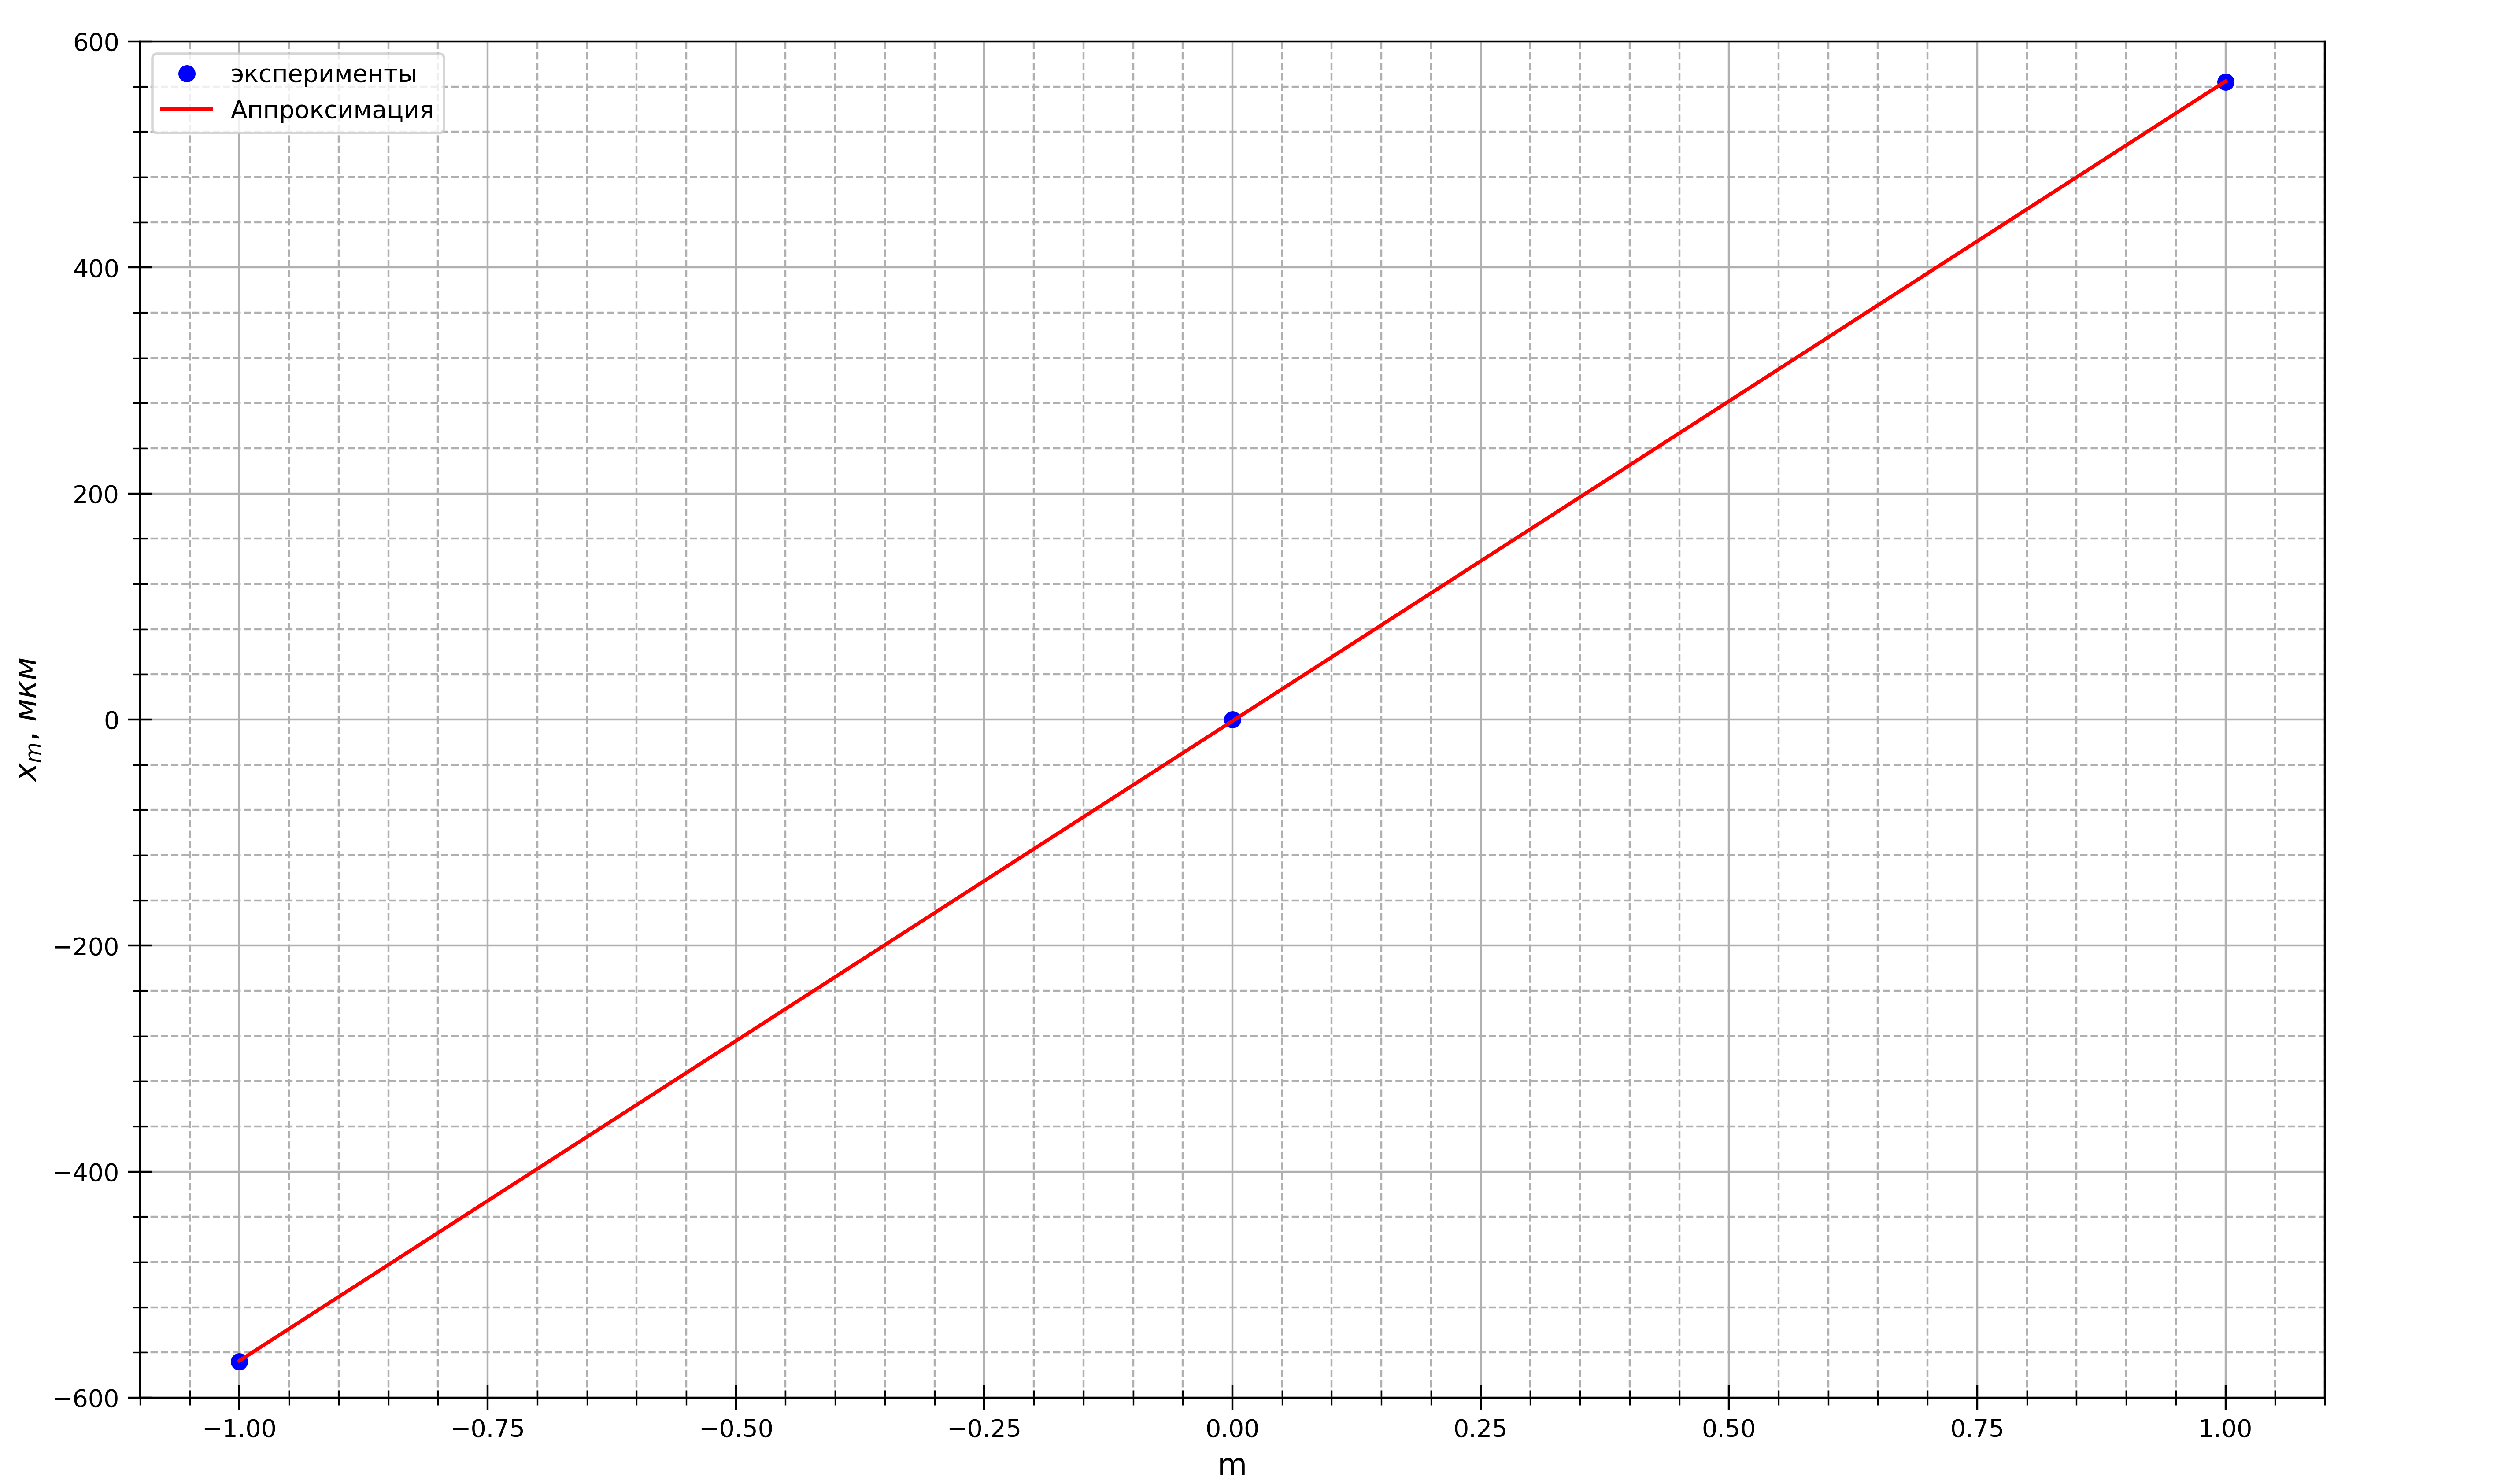
\includegraphics[width=0.7\textwidth]{graph4.png}
		\caption{Координаты $ m $-ого максимума $ x_m $ дифракционной картины при частоте генератора $ \nu = $ 4,615 МГц}
		\label{diff}
	\end{figure}
\begin{center}
    $v_4= 1565\pm 55$ м/c
\end{center}
\newpage 
\subparagraph{2.} Рассчитаем длину и скорость УЗ-волны в воде методом тёмного поля.\par
Проведем измерение длины ультразвуковой волны, приняв ошибку равной цене деления окулярной шкалы. В таблице 6 содержатся количество маленьких делений окулярной шкалы N (цена деления $ C = 0,8 $), соответствующее $ n $ темным полосам акустической решетки.
Формулы для расчета длины волны ультразвука $ \Lambda $ и скорости распространения $ v $ в воде:
\begin{equation}\label{}
\Lambda/2  = NC/(n - 1),  \qquad v = \nu\Lambda
\end{equation}

Расчеты также приведены в таблице 5. Ошибка при таком определении скорости звука больше, чем в первой части работы, и
составляет около 5\%.

\begin{table}[!h]
\begin{center}
\begin{tabular}{|c|c|c|c|c|c|}
\hline
     $\nu$, Мгц & $N$ & $n$ & $\Lambda$, мм & $v$, м/c & $\Delta v$, м/c \\ \hline
     1,201 & 10 & 8 & 1,14 & 1373 & 69 \\ \hline
     1,036 & 9 &  6 & 1,60 & 1492 & 75 \\ \hline
     0,957 & 9 & 5 & 1,80 & 1723 & 86 \\ \hline
     1,088 & 10 & 7 & 1,33 & 1450 & 73 \\ \hline
    
\end{tabular}
\end{center}
\caption{Измерение координаты $ m $-ого максимума $ x_m $ дифракционной картины при частоте генератора $ \nu = $ 2,883 МГц}
\end{table}

\paragraph{Вывод:}В работе изучена дифракция света на акустической решетки, рассчитаны длина волны ультразвука и скорость его распространения в воде. Решетка наблюдалась методом
темного поля.


\end{document}
